%% Article/forum paper for the fuel monitoring thesis project.
\documentclass[10pt,journal]{IEEEtran}

\usepackage{amsmath}
\usepackage{amssymb}
\usepackage{array}
\usepackage{booktabs}
\usepackage{tabularx}
\usepackage[pdftex]{graphicx}
\usepackage{subcaption}% for side-by-side sub-figures (prototype/mobile/dashboard triptych)
\usepackage{placeins}% \FloatBarrier so a table pinned to a section actually renders inside that section
\usepackage{url}
\usepackage{xurl}% more break points for long URLs (mainly SAE-standard slugs)
\usepackage{xcolor}% load before hyperref so blue!60!black is defined
% NOTE: do NOT load the `cite' package here. `cite' rewrites the internal
% \@cite / \@citex commands after hyperref has already redefined them for
% linked citations, which removes the hyperlink from every [N] and every
% "[Online]. Available: https://doi.org/..." target in the IEEEtran
% References list. hyperref + IEEEtran already produce compressed [N]-style
% citations with working PDF hyperlinks on their own, so we keep hyperref as
% the last package loaded and skip \usepackage{cite}.
\usepackage{hyperref}

\graphicspath{{figure/}}

\hypersetup{
bookmarks=true,
bookmarksnumbered=true,
pdfpagemode={UseOutlines},
plainpages=false,
pdfpagelabels=true,
colorlinks=true,
allcolors=blue,
linkcolor=blue,
citecolor=blue,
urlcolor=blue,
breaklinks=true,
pdftitle={An IoT-Enabled System for Real-Time Fuel Monitoring, GPS Tracking, and Fuel Anomaly Detection in Trucks Using Context-Aware Non-Parametric Machine Learning},
pdfsubject={IoT-enabled fuel monitoring and anomaly detection},
pdfauthor={Samuelle P. Barja, Konrad Romel C. Castelo, Eliza Rica R. De La Rosa, and Alyssa S. Montemayor},
pdfkeywords={Fuel Monitoring, GPS Tracking, Fuel Anomaly Detection, Internet of Things, Context-Aware Machine Learning, Isolation Forest, Matrix Profile}
}

\newcolumntype{Y}{>{\raggedright\arraybackslash}X}

\begin{document}

\title{An IoT-Enabled System for Real-Time Fuel Monitoring, GPS Tracking, and Fuel Anomaly Detection in Trucks Using Context-Aware Non-Parametric Machine Learning}

\author{Samuelle~P.~Barja,
        Konrad~Romel~C.~Castelo,
        Eliza~Rica~R.~De~La~Rosa,
        and~Alyssa~S.~Montemayor%
\thanks{Manuscript submitted August~1,~2026.}%
\thanks{S.~P. Barja, K.~R.~C. Castelo, E.~R.~R. De~La~Rosa, and A.~S. Montemayor are with the Department of Electronics, Computer, and Electrical Engineering, Gokongwei College of Engineering, De~La~Salle University, Manila, Philippines (e-mail: samuelle\_barja@dlsu.edu.ph; konrad\_castelo@dlsu.edu.ph; eliza\_delarosa@dlsu.edu.ph; alyssa\_montemayor@dlsu.edu.ph).}}

\IEEEtitleabstractindextext{%
\begin{abstract}
Fuel accountability in delivery-truck operations requires more than a fuel gauge: it requires synchronized vehicle telemetry, route context, resilient communication, and an anomaly model that distinguishes abnormal fuel loss from traffic, idling, refueling, sender noise, and driver variability. This paper presents an implemented IoT-enabled fleet-monitoring prototype developed with Hino Para\~naque Subic GS Auto Inc. The system acquires OBD-II fuel, speed, GPS, trip-state, and alert data through an embedded HMI; transmits telemetry through LoRa, LTE/GSM, WiFi, and offline replay; stores records in a cloud backend; and detects fuel anomalies using context-aware non-parametric learning. The production detector is Isolation Forest Model~C, supported by Matrix Profile as a subsequence detector and by a data-mining layer for operating-regime interpretation. Fuel anomalies are modeled as context-conditioned deviations between observed and expected fuel-level change under speed, RPM, engine load, throttle, route, driver, and motion state. Field and controlled-injection evaluation showed 1.04\% MAPE fuel accuracy, 5.52~s median GPS sampling, 90.21\% GPS fix availability, 92.9\% precision and 1.09\% false-positive rate for Model~C under leave-one-trip-out validation, and a 95.0\% alert-resolution rate. The results support the use of context-aware telemetry and interpretable anomaly signatures for practical fleet fuel monitoring, while parked-depot siphoning remains a future-work boundary requiring a dedicated stationary-state detector.
\end{abstract}

\begin{IEEEkeywords}
Context-aware machine learning, fuel anomaly detection, Internet of Things, Isolation Forest.
\end{IEEEkeywords}}

\maketitle
\IEEEdisplaynontitleabstractindextext
\IEEEpeerreviewmaketitle
% IEEEtran's \maketitle sets up "Barja et al.: <title>" as the running-head
% mark via its default page-style machinery. Force a plain short-title
% header on every subsequent page by (a) redefining \ps@headings so the
% page-style hook produces our title without any author prefix, and (b)
% re-issuing \pagestyle{headings} so LaTeX picks the new definition up.
% Build a two-line header that shows the FULL title. Line 1 = first half of
% the title, line 2 = second half + page number. Using \shortstack keeps the
% two lines centered inside the header box; we also grow \headheight so the
% two-line stack does not clash with the body text.
\newcommand{\ArticleHeaderA}{An IoT-Enabled System for Real-Time Fuel Monitoring, GPS Tracking, and Fuel Anomaly}
\newcommand{\ArticleHeaderB}{Detection in Trucks Using Context-Aware Non-Parametric Machine Learning}
\setlength{\headheight}{22pt}
\setlength{\headsep}{16pt}
\makeatletter
% First reset any per-page style hook to our custom header (two lines,
% right-aligned page number on odd pages, left-aligned on even).
\renewcommand{\ps@headings}{%
  \def\@oddhead{\hbox{}\@IEEEheaderstyle
    \parbox[b]{\dimexpr\textwidth-2em\relax}{\raggedright \MakeUppercase{\ArticleHeaderA}\\ \MakeUppercase{\ArticleHeaderB}}%
    \hfil\raisebox{-\baselineskip}{\thepage}}%
  \def\@evenhead{\@IEEEheaderstyle\raisebox{-\baselineskip}{\thepage}\hfil
    \parbox[b]{\dimexpr\textwidth-2em\relax}{\raggedright \MakeUppercase{\ArticleHeaderA}\\ \MakeUppercase{\ArticleHeaderB}}%
    \hbox{}}%
  \let\@oddfoot\@empty
  \let\@evenfoot\@empty
}
% ...then activate it AND directly overwrite \@oddhead/\@evenhead so the
% current page's shipout uses our custom header (\pagestyle only takes
% effect for the NEXT page, but the current page's shipout already has
% cached versions of \@oddhead/\@evenhead from IEEEtran's own setup).
\pagestyle{headings}
\def\@oddhead{\hbox{}\@IEEEheaderstyle
  \parbox[b]{\dimexpr\textwidth-2em\relax}{\raggedright \MakeUppercase{\ArticleHeaderA}\\ \MakeUppercase{\ArticleHeaderB}}%
  \hfil\raisebox{-\baselineskip}{\thepage}}
\def\@evenhead{\@IEEEheaderstyle\raisebox{-\baselineskip}{\thepage}\hfil
  \parbox[b]{\dimexpr\textwidth-2em\relax}{\raggedright \MakeUppercase{\ArticleHeaderA}\\ \MakeUppercase{\ArticleHeaderB}}%
  \hbox{}}
\let\@oddfoot\@empty
\let\@evenfoot\@empty
% Also override the title-page style so page 1 also uses the two-line header
\renewcommand{\ps@IEEEtitlepagestyle}{%
  \def\@oddhead{\hbox{}\@IEEEheaderstyle
    \parbox[b]{\dimexpr\textwidth-2em\relax}{\raggedright \MakeUppercase{\ArticleHeaderA}\\ \MakeUppercase{\ArticleHeaderB}}%
    \hfil\raisebox{-\baselineskip}{\thepage}}%
  \def\@evenhead{\@IEEEheaderstyle\raisebox{-\baselineskip}{\thepage}\hfil
    \parbox[b]{\dimexpr\textwidth-2em\relax}{\raggedright \MakeUppercase{\ArticleHeaderA}\\ \MakeUppercase{\ArticleHeaderB}}%
    \hbox{}}%
  \let\@oddfoot\@empty
  \let\@evenfoot\@empty
}
\thispagestyle{headings}
\makeatother
\markboth{\ArticleHeaderA\ \ArticleHeaderB}{\ArticleHeaderA\ \ArticleHeaderB}

\section{Introduction}
\IEEEPARstart{F}{uel} cost, fuel theft, unreported leakage, poor route visibility, and delayed alert response remain persistent problems in delivery-fleet operations. Traditional approaches treat fuel monitoring, Global Positioning System (GPS) tracking, and driver alerts as separate functions, so a fuel drop cannot be reconciled against traffic-idling, sender noise, refueling recovery, or driver style. Prior Internet of Things (IoT) fuel-monitoring systems remain hardware-only or rule-driven, while machine-learning (ML) studies on heavy vehicles frequently use datasets detached from an integrated field prototype~\cite{mumcuoglu2023fuel}. In the Philippine setting, fuel accountability is compounded by dense Metro Manila traffic, informal fuel-market pressure, and cargo-route restrictions~\cite{jica2022metro_traffic,adb2016fuel_smuggling}.

This study implements and evaluates a complete edge-to-cloud truck-monitoring system developed with Hino Para\~naque Subic GS Auto Inc.~(SGSA). It combines On-Board Diagnostics-II (OBD-II) fuel and engine telemetry, GPS tracking, prioritised communication, cloud storage, in-cab Human-Machine Interface (HMI) and mobile trip controls, and context-aware anomaly detection. The contributions are (1)~an integrated IoT fuel/GPS/alerting prototype; (2)~a context-conditioned anomaly model grounded in physical and operational constraints; (3)~an Isolation Forest (IF)~\cite{liu2008isolation_forest} production detector supported by Matrix Profile (MP)~\cite{yeh2016matrix_profile} and K-Means archetype discovery; and (4)~a per-SO evaluation across fuel accuracy, communication reliability, GPS cadence, anomaly detection, and alert usability. Because dipstick calibration and tank modification were not permitted, the design used non-invasive OBD-II / Engine Control Unit (ECU) acquisition and known-volume pump-gas events as the SO1 reference. The communication design uses multiple radio paths --- Long-Range low-power radio (LoRa), Long-Term Evolution (LTE), Global System for Mobile Communications (GSM) fallback, and IEEE~802.11 WiFi --- with local replay.

\section{Related Work}
\textbf{IoT fleet-monitoring and fuel-specific systems.} A large body of work has established that GPS, GSM/WiFi backhaul, cloud dashboards, and low-cost tank sensors can expose vehicle and fuel telemetry to a fleet back-office~\cite{mathi2024development}. Fuel-specific implementations typically raise theft or low-fuel alarms from resistive, ultrasonic, or capacitive sender readings crossing a static threshold. The engineering weakness that runs through both lines of work, and through commercially available platforms~\cite{samsara2026fuel_management}, is that a fuel drop is treated as self-explanatory: a per cent threshold fires an alarm without reconciling the drop against engine work, road grade, driver style, or post-refuel settling. A drop while idling in city traffic, climbing under load, or settling after a refuel is not the same event as siphoning, and threshold-only pipelines have no mechanism to say so.

\textbf{Machine-learning approaches to fuel anomalies.} Recent work reframes abnormal fuel consumption as a multivariate anomaly-detection problem. Mumcuoglu \textit{et al.}~\cite{mumcuoglu2023fuel} classify fuel-consumption anomalies on heavy-duty vehicles, and Turan \textit{et al.}~\cite{turan2024detecting} combine unsupervised detectors in an ensemble for the same class. Barbado and Corcho~\cite{barbado2022interpretable} argue explicitly that a fleet-facing detector must explain \emph{why} a point is anomalous rather than merely output a score, and Hirth \textit{et al.}~\cite{hirth2025truck_survey} survey the truck-anomaly field and identify the same gap the present work addresses: interpretable, context-aware, deployable detectors remain rare in commercial truck fleets.

\textbf{Similar studies and our novelty.} Three prior studies are the closest match to the present work in scope. Mathi \textit{et al.}~\cite{mathi2024development} developed a fuel-monitoring and theft-detection system for a delivery truck built around GPS/GSM telemetry, but the detection layer is rule-based on raw fuel level and does not condition on driver, route, or engine context. Turan \textit{et al.}~\cite{turan2024detecting} apply an ensemble of unsupervised anomaly detectors to high fuel consumption in heavy-duty vehicles and achieve strong detection rates on a large corpus, but the study is offline and no field prototype, HMI, or alert pipeline is deployed. Barbado and Corcho~\cite{barbado2022interpretable} focus on interpretable ML for fuel-consumption anomalies and are the closest match on the interpretability axis, but their deployment target is a fleet-analytics dashboard rather than an in-cab HMI and mobile companion tied to a live alert loop. The novelty of the present work is that it combines all three axes at once --- the deployment scope of Mathi \textit{et al.}, the multivariate anomaly-detection approach of Turan \textit{et al.}, and the interpretability discipline of Barbado and Corcho --- into one integrated field prototype validated on a Philippine partner fleet vehicle, with per-flag constraint tagging that lets an operator defend every alert to the driver.

\section{Standards and Design Constraints}
\label{sec:art_standards}
The prototype was designed against a set of technical standards applied as design constraints at design time; third-party conformity assessment was outside the scope of this prototype. Vehicle acquisition and sampling follow ISO~15765-4~\cite{iso15765_4} together with ISO~15031-5 and SAE~J1349, which jointly fix OBD-II CAN acquisition and the $\Delta s = 1.5$~s sampling interval. Peripheral discipline follows IEEE~1451 (UART NMEA GPS parsed as ASCII enables backend fusion with the mobile-app GPS fallback), and hardware robustness follows IEC~61131-2, ISO~7637-2, and CE/FCC marking (watchdog scan-loop firmware, SPIFFS offline buffer surviving reset, CE/FCC-marked variants, LoRa bounded to 433~MHz/SF7/125~kHz/17~dBm). Wide-area link selection follows Philippine NTC MC No.~003-09-2025~\cite{ntc2025legacy_network_phaseout}: LTE Cat-1 as primary with GSM~2G as transitional fallback. Transport and security follow RFC~791, IEEE~802.11, and ISO/IEC~27001~\cite{iso27001}: IP-over-TCP shared across LTE/GSM/WiFi with mandatory HTTPS/TLS. Software architecture follows ISO/IEC/IEEE~42010~\cite{iso42010} with a five-layer decomposition and explicit interface contracts (inference relocatable from the ESP32 to the backend), and the test discipline follows ISO/IEC~29119 (controlled injection, LOTO cross-validation, out-of-distribution clean condition). Data protection follows ISO/IEC~27018 and GDPR (opaque driver identifiers, row-level security, role-scoped views); system authority is bounded by ISO~26262, ISO~39001, and ISO~45001 (read-only vehicle-bus access, advisory-only driver output, non-invasive installation). AI accountability follows IEEE~P7003~\cite{ieeep7003}: alerts carry contextual evidence rather than opaque scores, and the refuel/quiescence contextual gate is documented.

\section{Objectives and Evaluation}
\label{sec:art_objectives}
The study was organised around one general objective (GO) and five specific objectives (SOs). The GO is to develop and evaluate an IoT-based system for trucks, in collaboration with SGSA, that monitors real-time fuel levels, tracks routes using GPS, and detects unusual fuel consumption using ML, with the goal of improving driver safety, supporting rest scheduling, and facilitating proactive vehicle maintenance through automated alerts. The five SOs are:
\begin{itemize}
    \item \textbf{SO1:} Non-invasive fuel measurement via OBD-II/ECU within $\pm$5\% real-time accuracy.
    \item \textbf{SO2:} Real-time fuel and GPS telemetry through IoT-based communication to a cloud server with a centralised dashboard.
    \item \textbf{SO3:} 5-second GPS logging correlated with route, fuel, and time context.
    \item \textbf{SO4:} Context-aware non-parametric anomaly-detection model (MP or IF) achieving 90\% precision and 10\% FPR in controlled environments.
    \item \textbf{SO5:} Hardware-backed rest and maintenance alert mechanisms tied to the dashboard using cumulative fuel and distance data.
\end{itemize}

Table~\ref{tab:article-task-summary} summarises the per-SO targets and headline results, with the detailed data tables presented per-SO in Section~\ref{sec:art_results_so1}~onward.

\begin{table}[!htbp]
\centering
\caption{Task Evaluation Summary (SO1--SO5, all met)}
\label{tab:article-task-summary}
\scriptsize
\setlength{\tabcolsep}{2pt}
\renewcommand{\arraystretch}{1.05}
\begin{tabularx}{\columnwidth}{@{}p{0.06\columnwidth}Y Y@{}}
\toprule
\textbf{SO} & \textbf{Target} & \textbf{Measured} \\
\midrule
1 & $\pm$5\% accuracy & 1.04\% MAPE; 3.00\% max err \\
2 & Real-time cloud telemetry & LoRa/LTE/GSM/WiFi + SPIFFS replay \\
3 & 5 s GPS logging & 5.52~s median, 90.21\% fix \\
4 & $\geq$90\% P, $\leq$10\% FPR & IF Model~C: 92.9\% P, 1.09\% FPR \\
5 & Usable alerts + interface & 100 alerts, 95\% resolved, SUS 81.9 \\
\bottomrule
\end{tabularx}
\normalsize
\end{table}
\FloatBarrier

\section{System Architecture}
Fig.~\ref{fig:end-to-end-architecture} shows a layered edge-to-cloud architecture per ISO/IEC/IEEE~42010~\cite{iso42010}: an edge layer (OBD-II acquisition, GPS parsing, fuel filtering, trip-state handling, HMI, channel selection), a transport layer (prioritised LoRa/LTE/GSM/WiFi with SPIFFS offline replay), and a cloud layer (Supabase Postgres storage, backend rules and anomaly inference, synchronised dashboard/mobile/HMI views).

\begin{figure}[!t]
\centering
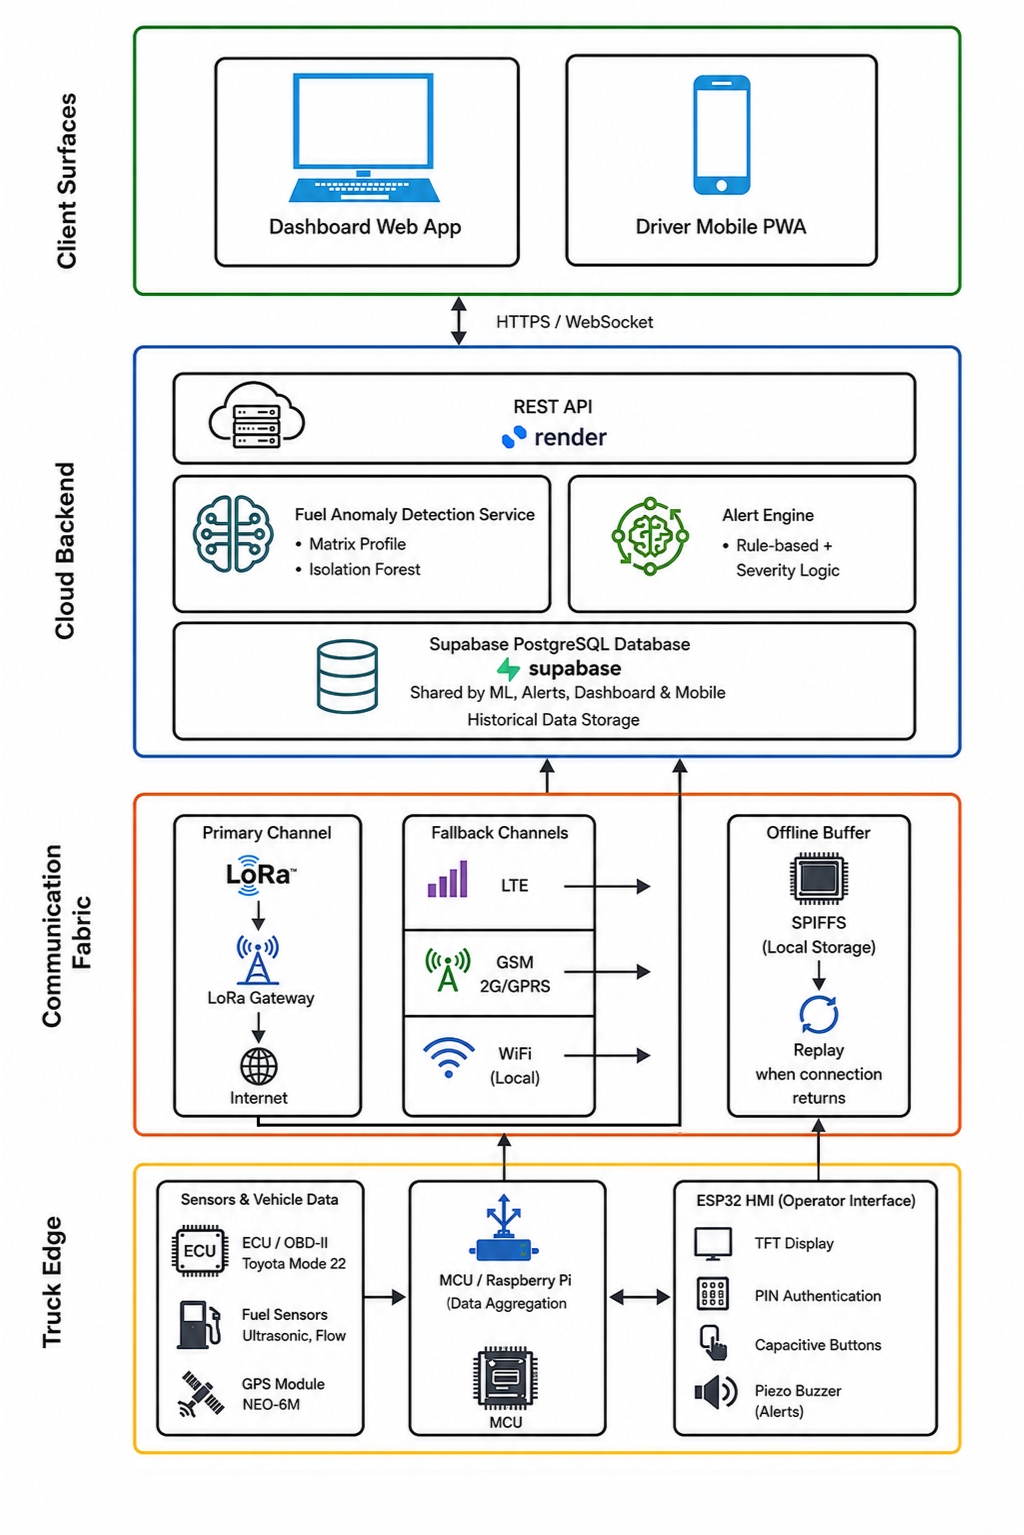
\includegraphics[width=\columnwidth]{systemArchi}
\caption{End-to-end edge-to-cloud system architecture with the ESP32-based in-cab hardware block.}
\label{fig:end-to-end-architecture}
\end{figure}

\emph{Hardware.} An ESP32-WROOM-32 MCU (dual-core, 240~MHz, FreeRTOS + Espressif IDF) coordinates all peripherals. The CAN interface is an MCP2515 + SN65HVD230 for OBD-II Mode~01 and manufacturer Mode~22 access per ISO~15765-4~\cite{iso15765_4} and ISO~15031-5; fuel level is read via Mode~22 PID~21/29 at 0.5~L per ADC count. The HMI is an ILI9341 2.4-inch TFT + XPT2046 touch with physical buttons for safety-critical actions per ISO~45001. Wide-area comms use an A7670E LTE Category-1 modem with GSM~2G fallback per NTC MC No.~003-09-2025~\cite{ntc2025legacy_network_phaseout}; depot comms use an SX1278 LoRa radio at 433~MHz / SF7 / 125~kHz / 17~dBm~\cite{devalal2018lora}. The GNSS receiver is a u-blox NEO-M8N on UART at 9600~baud reporting NMEA~0183; a mobile-app GPS stream is fused at the backend. Local persistence is a SPIFFS ring buffer surviving ISO~7637-2 transient resets.

\emph{Backend and database.} Node/Express on Render backed by Supabase Postgres. The trip session is the canonical state object; schema tables include \texttt{trucks}, \texttt{drivers} (opaque IDs per ISO/IEC~27018), \texttt{trips} (start/rest/resume/end with device- and backend-side timestamps), \texttt{telemetry\_logs} (raw and filtered fuel level, GPS, speed, engine load, RPM, throttle, MAF, coolant, runtime, \texttt{channel\_used}), \texttt{alerts} (five classes with a lifecycle state machine), and audit tables. Row-level security is enforced at the database layer; dashboard views are role-scoped. HTTPS/TLS is common across LTE, GSM, and WiFi per ISO/IEC~27001~\cite{iso27001} and RFC~791.

\emph{Alert engine.} Five rule classes fire in the backend: fuel-anomaly (Model~C + MP survives the contextual gate and clears the combined-score threshold), overspeed (GPS instantaneous speed exceeds per-route limit), low-fuel (filtered level below threshold under motion), rest (cumulative continuous driving time), and maintenance (cumulative distance). Every alert is mirrored to the HMI (buzzer + banner), mobile app (push + inbox), and dashboard (map pin + list). Rest and maintenance alerts require driver acknowledgement, logged back for latency/resolution audit.

\section{Methodology}
\subsection{Telemetry Acquisition and Filtering}
Fuel, speed, GPS, trip, and engine data are sampled by the HMI and transmitted as synchronised telemetry rows. The main OBD-II and ECU-derived fields include fuel level, speed, RPM, engine load, throttle position, mass airflow, coolant temperature, runtime, and diagnostic status. Fuel level is the primary measurement for SO1 and SO4, while the remaining fields provide the operating context needed to judge whether a fuel change is plausible.

Fuel readings are filtered before model inference. The median--exponential moving average (EMA)--dead-band--direction-aware cascade is grounded in classical digital signal processing (DSP) practice~\cite{oppenheim2010dsp} and robust statistics.


\emph{Stage~1: median rejection.} The Stage-1 output is the rank-order statistic
\begin{equation}
m_t = \operatorname{median}\bigl(x_{t-W+1},\, x_{t-W+2},\, \ldots,\, x_t\bigr),\quad W = 31
\label{eq:art-median}
\end{equation}
with a $W = 31$-sample window ($\approx 46.5$~s memory at the $\Delta_s = 1.5$~s cadence). The median has a 50\% breakdown point, so a single 5~L slosh spike leaves $m_t$ unchanged as long as fewer than 15 of the last 31 samples are contaminated.

\emph{Stage~2: first-order infinite-impulse-response (IIR) EMA.} The Stage-2 output is
\begin{equation}
y_t = \alpha\, m_t + (1 - \alpha)\, y_{t-1},\quad \alpha = 0.04
\label{eq:art-ema}
\end{equation}
whose equivalent time constant and 95\% step-response settling time follow from~\cite{oppenheim2010dsp}:
\begin{equation}
\tau = \frac{-\Delta_s}{\ln(1-\alpha)} \approx 36.7\text{ s},\quad t_{95} \approx 3\tau \approx 110\text{ s}.
\label{eq:art-ema-time-constant}
\end{equation}

\emph{Stages~3--4: dead-band + direction-aware.} The published anchor $p_t$ updates from $y_t$ only when $|y_t - p^{a}_{t-1}| \geq \theta_{\mathrm{db}}(s_t)$, with $\theta_{\mathrm{db}} = 0.5\%$ moving and $1.5\%$ stationary. A direction-aware rule enforces that fuel cannot rise mid-motion: $p_t{=}y_t$ if $\Delta_t \leq -2.5\%$ (down: real burn) or if $\Delta_t \geq +10\%$ and $T_{\mathrm{park}}\geq60$~s (up: gated refuel); otherwise $p_t{=}p^{a}_{t-1}$.

\emph{Kalman-filter alternative.} A physics-aware Kalman filter~\cite{kalman1960new} was implemented as a comparison stream (predict $\hat{x}_{t|t-1} = \hat{x}_{t-1|t-1} - u_t\Delta_s$, update with gain $K_t = P/(P+R)$), with $Q$ calibrated from parked-hour drift and $R$ from post-EMA moving-cruise residuals. It is evaluated against the EMA cascade in Section~\ref{sec:art_results_so1}.

Fuel accuracy was evaluated against pump-gas reference events and the known tank capacity. The primary accuracy metric was the mean absolute percentage error (MAPE):
\begin{equation}
\mathrm{MAPE} = \frac{100}{n}\sum_{i=1}^{n}\left|\frac{V_{\mathrm{sensor},i}-V_{\mathrm{ref},i}}{V_{\mathrm{ref},i}}\right|.
\label{eq:art-mape}
\end{equation}

\subsection{Fuel-Anomaly Model}
A fuel anomaly is modeled as a telemetry row whose observed fuel-level change deviates from the expected fuel-level change under operating context. For row $t$,
\begin{equation}
A(t)=
\frac{\left|\Delta f_{\mathrm{obs}}(t)-\mathbb{E}[\Delta f\mid c(t)]\right|}
{\sigma(c(t))},
\label{eq:article-anomaly-model}
\end{equation}
where $c(t)$ includes speed, RPM, engine load, throttle, route, driver, and motion state. This makes the detector a context-conditioned fuel-deviation model rather than a simple sudden-drop detector.

Four physical constraints (C1 conservation, C2 bounded consumption per SAE~J1349, C3 sender non-linearity, C4 slosh) and four operational constraints (O1 traffic/idling, O2 route restrictions~\cite{jica2022metro_traffic}, O3 driver variability, O4 refuel patterns) encode the fleet-operation context and are implemented through direction-aware rules, refuel gates, fuel-per-RPM/load features, driver fuel-economy deviation, and post-refuel flags~\cite{barbado2022interpretable,turan2024detecting}.

\subsection{Machine Learning and Data Mining}
The production row-level detector is IF~\cite{liu2008isolation_forest} Model~C, chosen after ablating three feature sets: Model~A uses baseline fuel, motion, engine, and refuel-window features; Model~B adds driving-zone features; Model~C adds per-asset, per-driver, and route-type fuel-economy deviation features. MP~\cite{yeh2016matrix_profile} is retained as a subsequence audit for gradual-leak patterns that per-row detectors cannot see. The backend derives the 33-feature Model~C vector per 5-second row and feeds IF and MP in parallel; both paths converge on the contextual gate defined below, a combined-score threshold ($>0.65$), and a per-truck 5-minute dedup window before insertion into the \texttt{alerts} table.

\subsubsection{Isolation Forest scoring}
With average path length $E[h(\mathbf{x})]$ over $n_t$ isolation trees, the anomaly score is
\begin{equation}
s(\mathbf{x}, n) = 2^{-E[h(\mathbf{x})]/c(n)},\quad c(n) = 2H(n-1) - \tfrac{2(n-1)}{n},
\label{eq:art-if-score}
\end{equation}
where $H(k) = \ln k + \gamma$ and $\gamma \approx 0.5772$. Scores approach 1 as $E[h(\mathbf{x})]\to 0$ (highly isolable). Model~C is trained with $n_t = 300$ trees, sub-sample $n = 256$, and contamination $c_{\mathrm{IF}} = 0.015$; the deployed \texttt{if\_with\_margin} rule fires when $s(\mathbf{x}) \geq \tau + \delta$, $\delta = 0.005$.

\subsubsection{Matrix Profile discord}
For a subsequence $T_{i,\ell}$ of length $\ell$ in a time series $T$, the Matrix Profile value is
\begin{equation}
P_i = \min_{j\,:\,|i-j|\geq\ell}\, d_{\mathrm{znorm}}\bigl(T_{i,\ell},\, T_{j,\ell}\bigr),
\label{eq:art-mp-score}
\end{equation}
where $d_{\mathrm{znorm}}$ is the $z$-normalised Euclidean distance. A large $P_i$ indicates a discord. Model~C uses $\ell = 12$ samples (60~s) and $z$-threshold 2.0; the escalation path fires when $P_i \geq 4.0$ with $\Delta f < 0$, or $P_i \geq 2.0$ with $\Delta f \leq -2.0$~L.

\subsubsection{Contextual gate}
The five-stage gate that guards every flagged row is a Boolean predicate:
\begin{equation}
\begin{aligned}
G(t) = {}& \neg\bigl(\text{parkedRefuel} \,\vee\, \text{postRefuel} \\
         & \phantom{\neg\bigl(}\vee\, \text{loadSpike} \,\vee\, \text{coldStart}\bigr) \\
         & \wedge\, \text{suspiciousContext}.
\end{aligned}
\label{eq:art-gate}
\end{equation}

\subsubsection{Data mining layer}
K-Means with $K = 4$ is used only for archetype discovery over seven standardised operating features (filtered $\Delta$fuel, speed, engine load, idle-duration score, motion state, throttle, normalised RPM), used only for interpretation, not primary detection. Constraint-violation profiling tags each flagged row with the physical or operational constraint whose bound was crossed.

\subsection{Evaluation Protocol}
Fuel accuracy, communication reliability, GPS cadence, anomaly detection, and alert usability were evaluated according to the study's five objectives. SO4 anomaly-detection metrics were computed using leave-one-trip-out (LOTO) cross-validation~\cite{arlot2010survey} on the project-native partition so that each held-out trip was scored by models trained and calibrated on separate trips. The headline classifier metrics follow the standard definitions~\cite{fawcett2006roc}:
\begin{equation}
\begin{gathered}
\mathrm{Precision} = \tfrac{TP}{TP+FP},\quad \mathrm{Recall} = \tfrac{TP}{TP+FN},\\
\mathrm{FPR} = \tfrac{FP}{FP+TN},\quad F_1 = \tfrac{2\,\mathrm{Precision}\,\mathrm{Recall}}{\mathrm{Precision}+\mathrm{Recall}},
\end{gathered}
\label{eq:art-metrics}
\end{equation}
and headline proportions carry two-sided Wilson-score~\cite{wilson1927probable} 95\% intervals ($z = 1.96$). Performance was additionally reported on ROC and PR axes~\cite{fawcett2006roc}, and detector-versus-baseline differences were tested with the paired-comparison apparatus (McNemar~\cite{mcnemar1947note}, bias-corrected bootstrap~\cite{efron1994bootstrap}, and paired Wilcoxon signed-rank~\cite{wilcoxon1945individual} on per-trip $F_1$). Usability of the dashboard and mobile app was measured with the SUS. The SO4 corpus included project-native trips with controlled injected anomalies plus a public-clean stress partition used to check whether the detector remains quiet on clean-route data.

\section{Results and Discussion}
\subsection{SO1: Fuel Measurement}
\label{sec:art_results_so1}
The fuel subsystem reached 1.04\% MAPE and 3.00\% maximum error across the 13--98\% tank range, satisfying the $\pm$5\% target. The worst observed event remained two percentage points inside the allowed error band. The filtered-signal noise analysis also showed that residual noise was below 0.1\% across the reported tank bands, supporting the claim that the filter cascade suppresses short slosh, ADC jitter, and sender bounce before the value is shown or modelled.

\begin{table}[!htbp]
\centering
\caption{SO1 Consolidated Fuel-Measurement Result}
\label{tab:art-so1-consolidated}
\scriptsize
\setlength{\tabcolsep}{2pt}
\renewcommand{\arraystretch}{1.05}
\begin{tabular}{@{}c c c c c c@{}}
\toprule
\textbf{Pump \#} & \textbf{Pre (L/\%)} & \textbf{Pumped (L)} & \textbf{Realised (L/\%)} & \textbf{Err (L)} & \textbf{Err (\%)} \\
\midrule
1 & 10.40 / 13\% & 9.60 & 20.00 / 25\% & 0.00 & 0.00\% \\
2 & 20.00 / 25\% & 20.00 & 40.80 / 51\% & $+0.80$ & $+1.00\%$ \\
3 & 40.80 / 51\% & 20.00 & 63.20 / 79\% & $+2.40$ & $+3.00\%$ \\
4 & 63.20 / 79\% & 14.97 & 78.30 / 98\% & $+0.13$ & $+0.16\%$ \\
\midrule
\multicolumn{6}{@{}l@{}}{\textbf{Aggregate:} MAPE 1.04\% ($\leq$5\% target); max err 3.00\%; MAE 0.83~L;} \\
\multicolumn{6}{@{}l@{}}{$\sigma$ 1.36\%; 4/4 events within $\pm$5\%; filtered-signal noise $<$0.1\%.} \\
\midrule
\multicolumn{6}{@{}l@{}}{\textbf{Deployed filter:} moving average (MA) selected over Kalman.} \\
\multicolumn{6}{@{}l@{}}{Noise reduction: MA $4$--$5\times$ (driving), $4.7\times$ (idle); Kalman $1.05$--$1.4\times$.} \\
\multicolumn{6}{@{}l@{}}{Signal preservation on labelled steps: MA $0.39$; Kalman $0.96$.} \\
\multicolumn{6}{@{}l@{}}{Downstream $F_1$: MA $55.4\%$; Kalman $45.9\%$.} \\
\multicolumn{6}{@{}l@{}}{Paired Wilcoxon per-trip $F_1$: $W = 3.0$, $p = 0.313$ (not rejected).} \\
\bottomrule
\end{tabular}
\normalsize
\end{table}

The lower half of Table~\ref{tab:art-so1-consolidated} summarises the moving-average versus Kalman comparison~\cite{kalman1960new}. The moving average was chosen for three practical reasons. First, it removes sender noise much more aggressively (4--5$\times$ on driving, 4.7$\times$ on idle) than Kalman (1.05--1.4$\times$); the HMI and anomaly detector both need a stable signal, not sub-sample fidelity. Second, it produced a higher downstream $F_1$ (55.4\% vs.\ 45.9\%), because the Kalman predict step subtracts an expected fuel-burn term and can absorb a real anomaly as ``explained by the model,'' while the moving average cannot smooth a real drop away by mistake. Third, the paired Wilcoxon test on per-trip $F_1$~\cite{wilcoxon1945individual} did not reject the null ($W = 3.0$, $p = 0.313$), so the moving average is at worst statistically tied and strictly better on aggregate downstream detection. The Kalman filter is retained as the physics-aware alternative for future consumers that require sub-sample fidelity. Because dipstick validation was not permitted, the reported numbers are operational field accuracy, not laboratory tank calibration.

\subsection{SO2: Communication Performance}
The communication subsystem met SO2 because every path was exercised. LoRa~\cite{devalal2018lora} covered depot and LOS fallback; LTE~\cite{miyim2019lte_performance} was the main wide-area path (LTE Category-1 selected per NTC MC No.~003-09-2025~\cite{ntc2025legacy_network_phaseout}); GSM~2G~\cite{iec_gsm_tutorial} was the fringe fallback; WiFi was opportunistic; SPIFFS replay preserved outages. The tables below report RSSI, SNR, and CSQ (0--31, higher = stronger), with LOS/NLOS placement.

\begin{table}[!htbp]
\centering
\caption{SO2 Consolidated Communication Result}
\label{tab:art-so2-consolidated}
\scriptsize
\setlength{\tabcolsep}{2pt}
\renewcommand{\arraystretch}{1.05}
\begin{tabular}{@{}l c c c c c@{}}
\toprule
\multicolumn{6}{@{}l@{}}{\textbf{(a) LoRa distance test (SX1278, SF7, 125~kHz, 17~dBm, 100 pkts/band)}} \\
\midrule
\textbf{Dist.} & \multicolumn{2}{c}{\textbf{Environment}} & \textbf{RSSI (dBm)} & \textbf{SNR (dB)} & \textbf{Success} \\
\midrule
10~m & \multicolumn{2}{c}{Urban NLOS} & $-81.2$ & $5.48$ & 99.0\% \\
50~m & \multicolumn{2}{c}{Urban NLOS} & $-90.9$ & $-0.60$ & 97.0\% \\
100~m & \multicolumn{2}{c}{Urban NLOS} & $-91.6$ & $-4.59$ & 57.0\% \\
500~m & \multicolumn{2}{c}{Urban NLOS} & $-98.0$ & $-10.20$ & 4.0\% \\
1~km & \multicolumn{2}{c}{Open LOS} & $-98.9$ & $-6.49$ & 60.0\% \\
1~km & \multicolumn{2}{c}{Urban NLOS} & $-104.0$ & $-9.37$ & 12.0\% \\
5~km & \multicolumn{2}{c}{Open LOS (elev.)} & $-98.0$ & $-12.80$ & 1.0\% \\
\midrule
\multicolumn{6}{@{}l@{}}{\textbf{(b) GSM/LTE signal + HTTPS latency by location}} \\
\midrule
\textbf{Location} & \textbf{Net} & \textbf{$n$} & \textbf{CSQ} & \textbf{Succ.} & \textbf{$p_{95}$ ms} \\
\midrule
Metro urban (Makati) & LTE & 47 & 25.2 & 100.0\% & 4{,}147 \\
Highway corridor & LTE & 46 & 25.4 & 89.1\% & 7{,}377 \\
Tunnel / underpass & LTE & 56 & 22.1 & 98.2\% & 5{,}358 \\
Provincial (Batangas) & LTE & 117 & 17.4 & 99.1\% & 4{,}692 \\
Provincial (Batangas) & GSM & 16 & 8.1 & 68.8\% & 12{,}016 \\
\midrule
\multicolumn{6}{@{}l@{}}{\textbf{(c) Per-transport end-to-end latency (field-test telemetry, ms)}} \\
\midrule
\textbf{Transport} & \textbf{$n$} & \textbf{$p_{50}$} & \textbf{$p_{95}$} & \textbf{$p_{99}$} & \textbf{Max} \\
\midrule
LoRa & 150 & 7{,}397 & 43{,}456 & 213{,}950 & 287{,}259 \\
WiFi & 459 & 7{,}245 & 20{,}328 & 61{,}725 & 252{,}147 \\
LTE & 2{,}884 & 23{,}109 & 75{,}058 & 118{,}013 & 291{,}104 \\
Offline replay & 13 & 100{,}378 & 261{,}911 & 273{,}062 & 275{,}850 \\
\midrule
\multicolumn{6}{@{}l@{}}{\textbf{(d) Packet delivery over 11{,}709 field-test rows:} LoRa 2.8\%,} \\
\multicolumn{6}{@{}l@{}}{WiFi 5.5\%, LTE 24.8\%, GSM~2G 0.03\%, offline-buffer 55.6\%,} \\
\multicolumn{6}{@{}l@{}}{replayed from offline 11.3\%.} \\
\bottomrule
\end{tabular}
\normalsize
\end{table}

The engineering lesson is that latency and packet preservation are different questions: cellular latency can spike during renegotiation, but offline replay still protects the record --- 66.9\% of delivered telemetry transited the offline buffer.


\subsection{SO3: GPS Tracking and Route Context}
The GPS subsystem reached a 5.52~s median sampling interval and 90.21\% GPS fix availability. The median interval is close to the 5~s firmware target; the longer mean and tail are explained by real field behavior such as OBD polling, GPS parsing, packet construction, connectivity delay, and replayed telemetry.

GPS is not just for map display: the route trace supplies segment distance, movement state, speed context, and route-type tags to Model~C, which is why SO3 supports SO4. The 100\% \texttt{gps\_source}/\texttt{route\_type} propagation and the backend fusion of the mobile-app GPS fallback close the route-context chain end-to-end.

\subsection{SO4: Machine-Learning Detection}
\label{sec:art_results_so4}
For anomaly detection, Model~C was the strongest production detector because it considered fuel movement relative to driver, route, and operating context. It achieved 92.9\% precision, 92.9\% recall, and 1.09\% FPR on the project-native leave-one-trip-out~\cite{arlot2010survey} partition. The result satisfies the 90\% precision and 10\% FPR requirements while preserving Model~C as the deployable row-level detector. The paired McNemar $\chi^2$ test~\cite{mcnemar1947note} against the threshold-only baseline confirmed the improvement was not attributable to sampling variance, and the bias-corrected bootstrap~\cite{efron1994bootstrap} of the precision estimate placed a Wilson-score~\cite{wilson1927probable} 95\% interval strictly inside the SO4 target band.

\begin{table}[!htbp]
\centering
\caption{SO4 Consolidated Anomaly-Detection Result (LOTO, 634 rows)}
\label{tab:art-so4-consolidated}
\scriptsize
\setlength{\tabcolsep}{2pt}
\renewcommand{\arraystretch}{1.05}
\begin{tabular}{@{}p{0.40\columnwidth} c c c c c@{}}
\toprule
\multicolumn{6}{@{}l@{}}{\textbf{(a) Model A/B/C feature-set ablation (IF, LOTO)}} \\
\midrule
\textbf{Model (features)} & \textbf{Prec.} & \textbf{FPR} & \textbf{TP} & \textbf{FP} & \textbf{FN} \\
\midrule
A --- context baseline (24) & 87.8\% & 1.09\% & 43 & 6 & 42 \\
B --- A + driving zones (30) & 88.9\% & 1.28\% & 56 & 7 & 29 \\
\textbf{C --- B + fuel-econ dev. (33)} & \textbf{92.9\%} & \textbf{1.09\%} & \textbf{79} & \textbf{6} & \textbf{6} \\
\midrule
\multicolumn{6}{@{}l@{}}{\textbf{(b) Detector configurations and baselines}} \\
\midrule
\textbf{Configuration} & \textbf{Prec.} & \textbf{Rec.} & \textbf{$F_1$} & \textbf{FPR} & \textbf{TP} \\
\midrule
Physics tripwire only & 73.1\% & 57.6\% & 64.5\% & 3.28\% & 49 \\
Static thr.\ $|\Delta f|{\geq}1\%$ & 100\% & 7.1\% & 13.2\% & 0.00\% & 6 \\
IQR fuel/km (Tukey~1.5$\times$) & 76.7\% & 92.9\% & 84.0\% & 4.37\% & 79 \\
IQR fuel $\Delta$ (Tukey~1.5$\times$) & 97.7\% & 100\% & 98.8\% & 0.36\% & 85 \\
Local Outlier Factor & 85.7\% & 98.8\% & 91.8\% & 2.55\% & 84 \\
Matrix Profile only (trip) & 100\% & 83.3\% & 90.9\% & 0.00\% & --- \\
IF $\cup$ MP hybrid union & 78.2\% & 92.9\% & 84.9\% & 4.01\% & 79 \\
IF $\cap$ MP hybrid inter. & 97.4\% & 89.4\% & 93.2\% & 0.36\% & --- \\
\textbf{IF Model~C (production)} & \textbf{92.9\%} & \textbf{92.9\%} & \textbf{92.9\%} & \textbf{1.09\%} & \textbf{79} \\
\bottomrule
\end{tabular}
\normalsize
\end{table}

Two statistical baselines in Table~\ref{tab:art-so4-consolidated}(b) actually score higher than Isolation Forest on this corpus --- IQR-on-fuel-$\Delta$ reaches 97.7\% precision at 100\% recall, and Local Outlier Factor reaches 98.8\% recall --- yet Isolation Forest Model~C was still chosen as the deployed detector. The reasons are practical rather than statistical. First, the two statistical baselines need to be re-tuned for every new truck (the IQR rule redraws its outlier cut-offs from that truck's own fuel-delta history), while Isolation Forest is tuned once against the SO4 target and can be reused across trucks. Second, Isolation Forest gives every row a clear anomaly score between 0 and 1 that the dashboard can display directly as a confidence value; IQR and LOF outputs are harder to interpret. Third, IEEE~P7003~\cite{ieeep7003} requires each alert to say \emph{why} it fired, and Isolation Forest lets each flagged row be tagged with the specific constraint that was crossed (for example, ``driver-baseline deviation'' or ``bounded consumption''). Fourth, Isolation Forest integrates cleanly with the contextual gate that filters out common false-positive causes such as post-refuel settling and load spikes. In short, Isolation Forest wins on reusability, interpretability, and integration --- not on raw accuracy alone. The Hybrid Intersection (97.4\% precision) is retained as an optional high-precision channel.


\subsection{SO5: Alerts, HMI, and Dashboard}
The alert subsystem completed the operator workflow. Alerts were surfaced across fuel anomaly, overspeed, low fuel, rest, and maintenance classes, with synchronised visibility across the HMI, mobile companion, and administrative dashboard. The field-test audit recorded 100 alerts over 17.7 days and a 95.0\% resolution rate.

Over the 17.7-day field-test window, 100 alerts were logged across all five classes with a 95.0\% resolution rate through the HMI/mobile/dashboard acknowledgement path. The administrator System Usability Scale (SUS) score of 81.9/100 ($n = 4$; one-sample Wilcoxon against the industry benchmark of 68 gives $p = 0.0625$ at the four-respondent exact-test floor) places the dashboard in the ``excellent'' band. Fig.~\ref{fig:art-so5-interfaces} shows the three operator-facing surfaces: the in-cab embedded HMI, the driver mobile application, and the fleet-administrator dashboard.

\begin{figure}[!htbp]
\centering
\begin{subfigure}[b]{0.31\columnwidth}
    \centering
    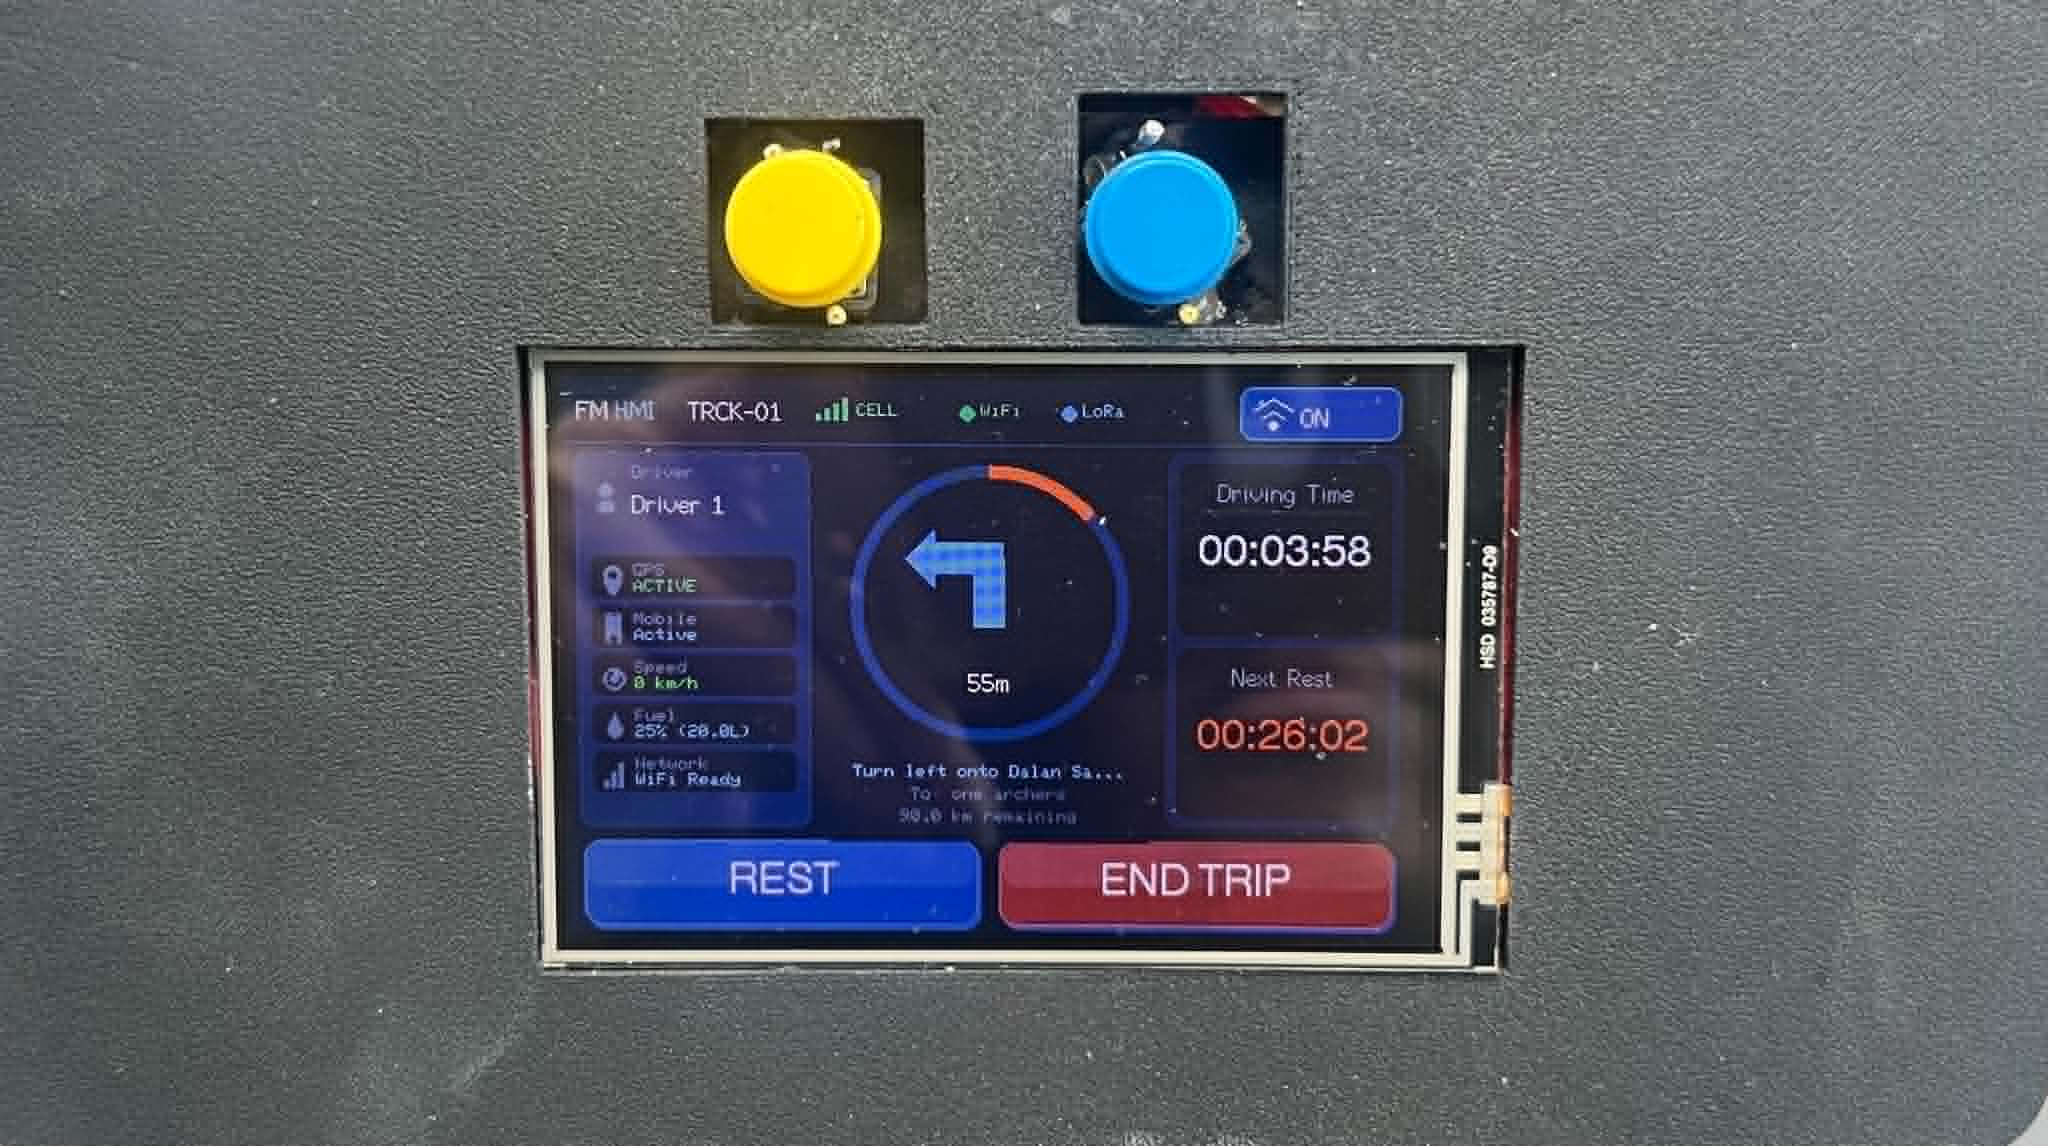
\includegraphics[width=\linewidth,height=3cm,keepaspectratio]{image23.jpg}
    \caption{HMI.}
    \label{fig:art-hmi}
\end{subfigure}\hfill
\begin{subfigure}[b]{0.31\columnwidth}
    \centering
    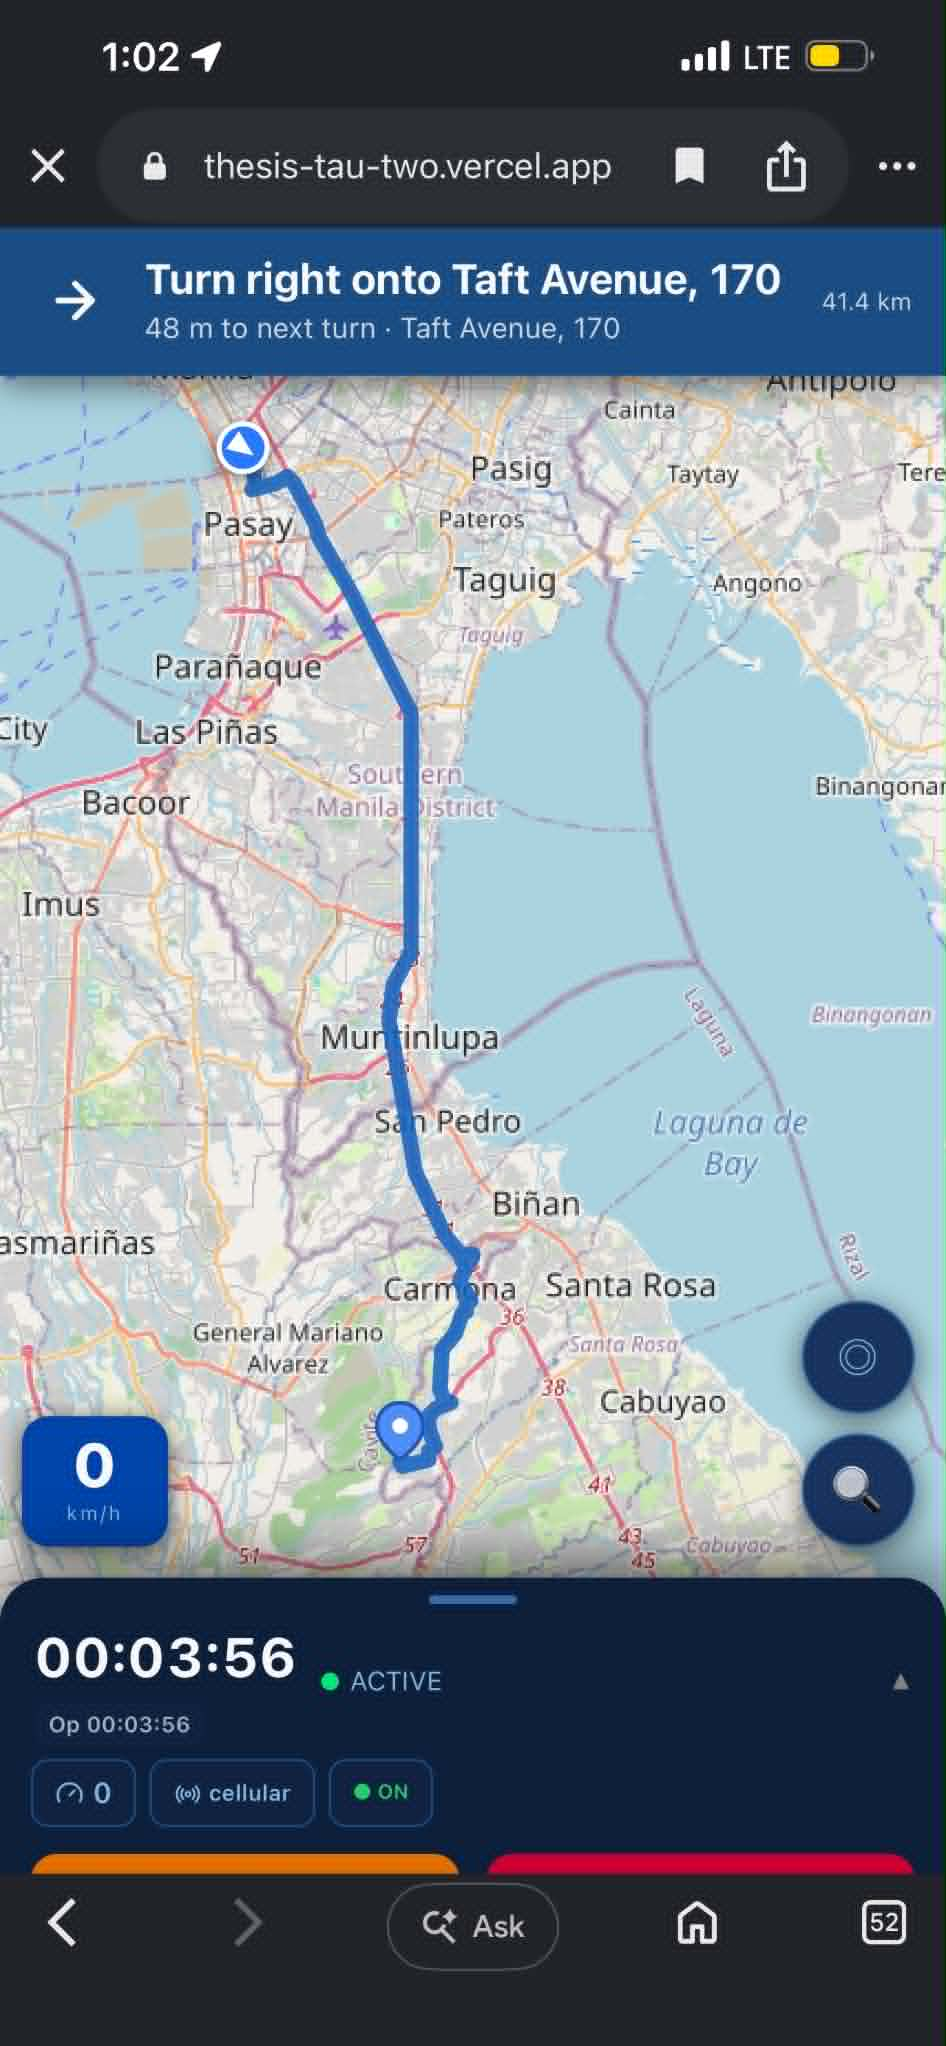
\includegraphics[width=\linewidth,height=3cm,keepaspectratio]{image7.jpg}
    \caption{Mobile.}
    \label{fig:art-mobile}
\end{subfigure}\hfill
\begin{subfigure}[b]{0.31\columnwidth}
    \centering
    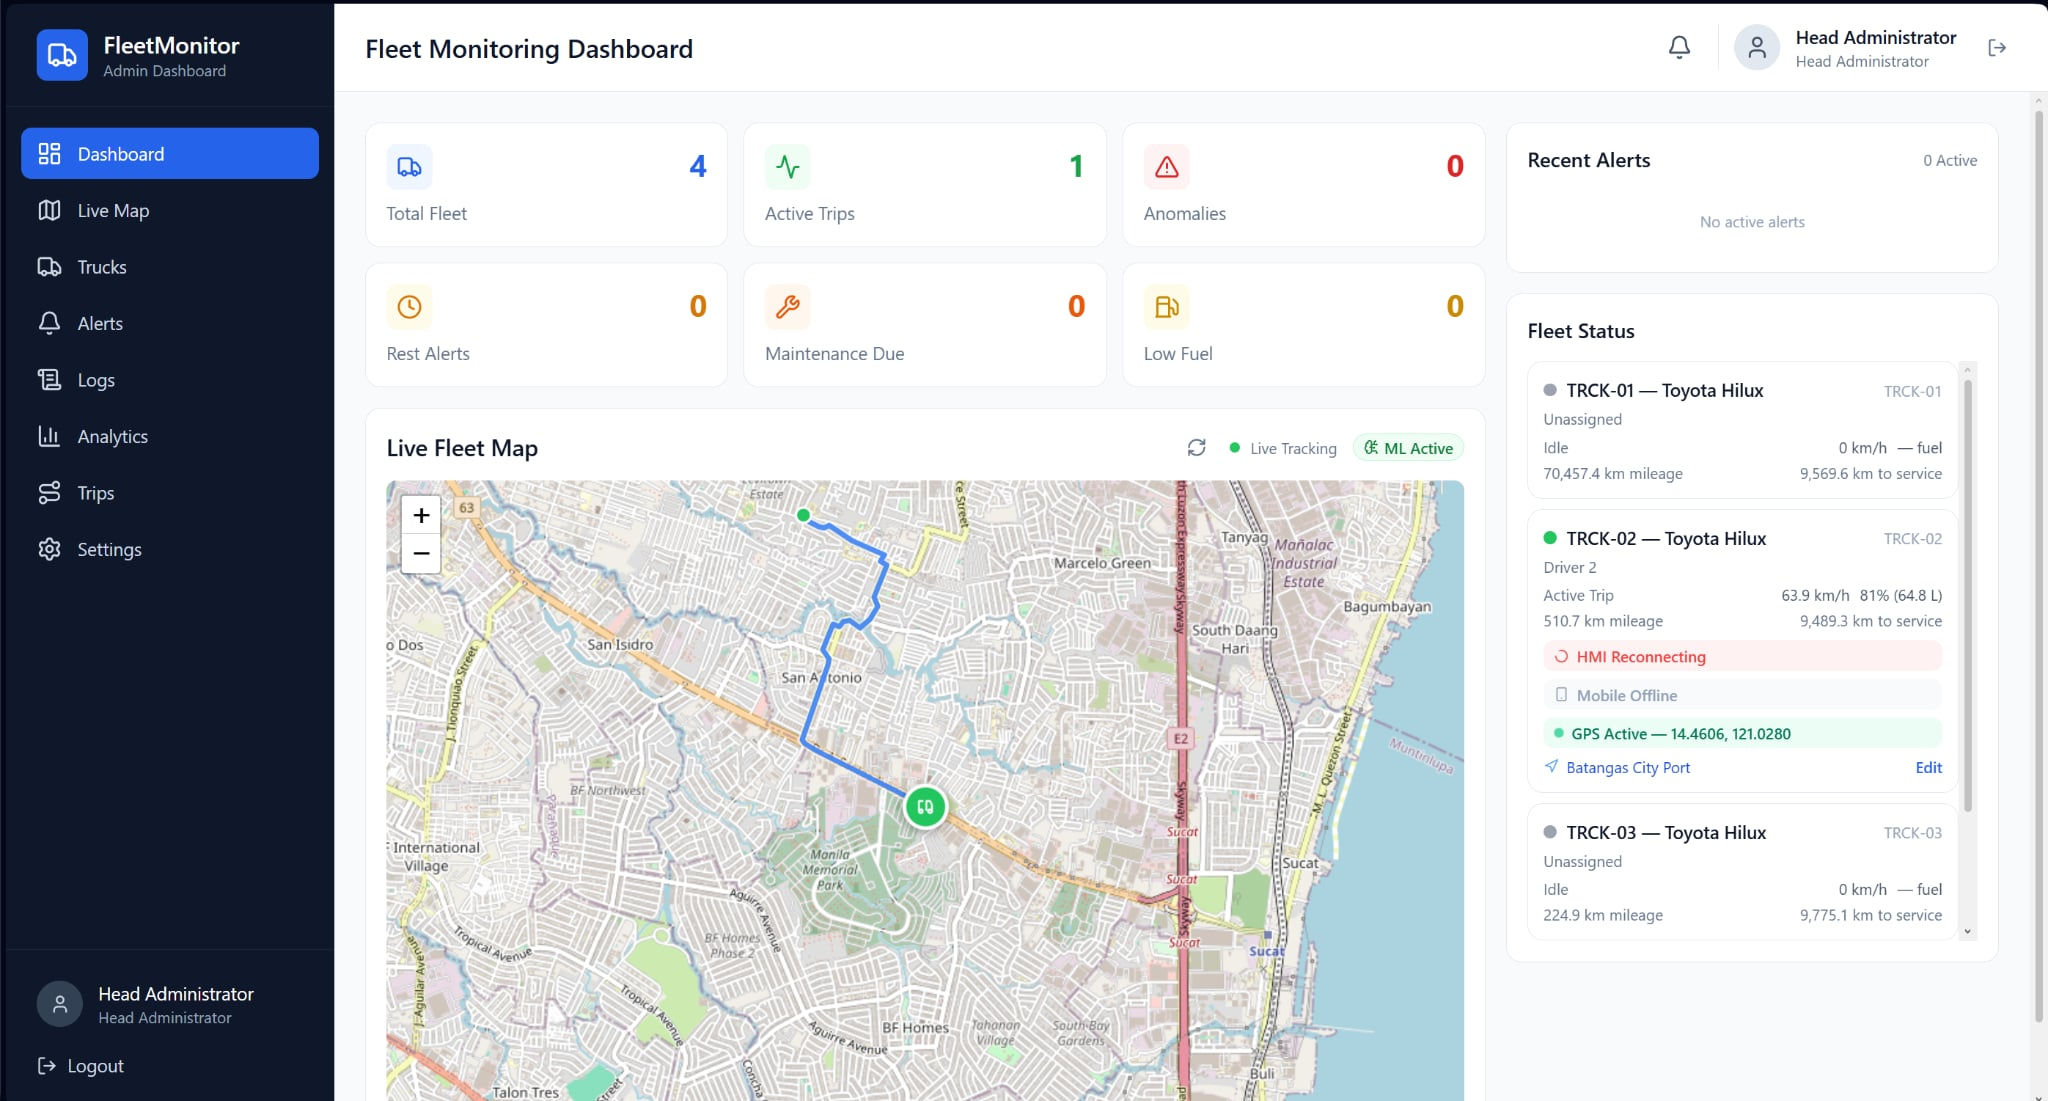
\includegraphics[width=\linewidth,height=3cm,keepaspectratio]{image26.jpg}
    \caption{Dashboard.}
    \label{fig:art-dashboard}
\end{subfigure}
\caption{SO5 operator interfaces: (a)~in-cab HMI on the active-trip page, (b)~driver mobile app on a long-haul route, and (c)~fleet-administrator dashboard.}
\label{fig:art-so5-interfaces}
\end{figure} This matters because a detector is operationally incomplete if alerts are not visible, persistent, and resolvable. The HMI, mobile app, and dashboard together support the loop from telemetry to event, from event to alert, and from alert to documented response. Data-privacy handling of driver identifiers, dashboard views, and location traces follows the ISO/IEC~27018 principles of opaque references, role-scoped views, and aggregate-only retention for reporting.

\subsection{Deployment, Ethics, and Scalability}
The field-test window ran for 17.7 continuous days on the partner SGSA vehicle across Metro-Manila-to-Batangas routes, producing 11{,}709 telemetry rows (66.9\% delivered via offline replay), 100 alerts across five rule classes, and a 95.0\% resolution rate. The study was approved by the DLSU URERB; driver identifiers are stored as opaque references per ISO/IEC~27018 and GDPR; and the prototype is strictly read-only on the vehicle CAN bus with advisory-only alerts. Beyond the single-vehicle pilot, Table~\ref{tab:art-scalability} projects the load on the deployed backend, LoRa gateway occupancy, and hot-table storage growth at four representative commercial fleet sizes ($N_v = 10, 100, 500, 1000$).

\begin{table}[!htbp]
\centering
\caption{Commercial-Scale Scalability Projection (per active vehicle)}
\label{tab:art-scalability}
\scriptsize
\setlength{\tabcolsep}{2pt}
\renewcommand{\arraystretch}{1.05}
\begin{tabular}{@{}p{0.42\columnwidth} c c c c@{}}
\toprule
\textbf{Metric} & \textbf{$N_v{=}10$} & \textbf{100} & \textbf{500} & \textbf{1000} \\
\midrule
Backend ingest rate (rows/s) & 2 & 20 & 100 & 200 \\
\% of shared-tier ceiling & 0.04\% & 0.4\% & 2.2\% & 4.3\% \\
LoRa gateways (60 nodes/gw) & 1 & 2 & 9 & 17 \\
Baseline storage (MB) & 0.04 & 0.4 & 2.0 & 4.0 \\
Hot-table growth (GB/day) & 0.04 & 0.36 & 1.80 & 3.60 \\
Hot-table growth (GB/month) & 0.79 & 7.92 & 39.6 & 79.2 \\
\midrule
\multicolumn{5}{@{}l@{}}{\textbf{First binding constraint:} LoRa gateway occupancy at $\approx$60} \\
\multicolumn{5}{@{}l@{}}{active nodes/gateway (sub-fleet grouping required $\geq N_v = 500$).} \\
\bottomrule
\end{tabular}
\normalsize
\end{table}

Three operational readings emerge from the projection. First, the shared-tier backend layer stays under 5\% of its ceiling even at $N_v = 1{,}000$, so ingest is comfortably provisioned across the full range considered. Second, LoRa gateway occupancy is the first binding constraint at commercial scale: at the ITU-recommended 30\% engineering occupancy, one gateway serves $\approx$60 active nodes, so a 500-vehicle depot requires nine gateways with distinct network identifiers, and a 1{,}000-vehicle deployment requires 17. Third, hot-table storage growth is a query-latency concern rather than a capacity one, and the archival cadence must be tightened from weekly to daily beyond $N_v \approx 500$ to keep the dashboard responsive.


\section{Limitations and Future Work}
The reported results have three principal limitations. First, they are drawn from a single-vehicle field deployment on the partner fleet vehicle, so extension to other makes requires a per-vehicle Mode~22 PID adapter and per-tank sender recalibration. Second, direct dipstick calibration was not permitted, so SO1 accuracy was validated against legally calibrated pump-gas events rather than a laboratory reference. Third, the SO4 labels were primarily controlled injected events rather than confirmed real-world theft incidents.

Future work therefore has four directions: (i)~multi-vehicle field deployment across additional makes and drivers, with sender recalibration formalised as a provisioning step and a dedicated stationary-state detector added for parked-depot siphoning; (ii)~migration to an LTE-only or 5G-capable modem as the Philippine 2G/3G phase-out~\cite{ntc2025legacy_network_phaseout} proceeds, and a re-evaluation of LoRa gateway occupancy beyond the boundary in Table~\ref{tab:art-scalability}; (iii)~deep-learning extensions surveyed by Hirth \textit{et al.}~\cite{hirth2025truck_survey} under the same interpretability discipline; and (iv)~hardening the unit-identification chain by binding each \texttt{truck\_id} to an immutable hardware anchor (ESP32 factory MAC or eFuse device ID) rather than a backend-issued UUID, tagging every telemetry payload with a firmware provenance stamp, and surfacing sensor-level identifiers on the dashboard for defensible data-quality attribution.

\section{Conclusion}
This paper presented an implemented IoT-enabled system for real-time truck fuel monitoring, GPS tracking, anomaly detection, and alert management, deployed on a partner Philippine delivery truck. The prototype met all five specific objectives: SO1, 1.04\% MAPE fuel accuracy against a legally calibrated pump reference; SO2, preserved telemetry delivery across a prioritised LoRa/LTE/GSM/WiFi stack backed by SPIFFS offline replay; SO3, 5.52~s median GPS sampling with 90.21\% fix availability; SO4, 92.9\% precision and 1.09\% false-positive rate under leave-one-trip-out validation for Isolation Forest Model~C~\cite{liu2008isolation_forest}; and SO5, 100 field-test alerts resolved at 95.0\% with an 81.9/100 administrator SUS score.

The central technical finding is that fuel anomalies must be modelled as context-conditioned deviations rather than as raw fuel drops. Isolation Forest Model~C, supported by the Matrix Profile~\cite{yeh2016matrix_profile} as a subsequence audit and by a constraint-aware data-mining layer, yields a production detector that is both operationally strong and auditable: every flagged row carries a physical or operational constraint signature, which is the property that lets a fleet operator defend an alert to a driver. Together with resilient prioritised communication, non-invasive OBD-II acquisition, and human-readable interfaces across the HMI, mobile application, and dashboard, the system demonstrates that fuel accountability and proactive fleet supervision are achievable with a documented, interpretable, and standards-compliant prototype in a real Philippine delivery-truck setting.

\section*{Acknowledgment}
The authors thank their thesis adviser Dr.~John Anthony Jose; panel members Dr.~Lawrence Materum (Chair), Dr.~Gerald Arada, and Dr.~Gerino Mappatao; thesis coordinators Dr.~Alexander Co Abad and Dr.~Ronnel Agulto; consultant Jayne Lois Go San Juan; the Department of Electronics, Computer, and Electrical Engineering of De~La~Salle University; the partner fleet operator Hino Para\~naque Subic GS Auto Inc.~(SGSA); Macaranas Percival~III Quinto and Guillarte Samuel John Deauna for materials and assistance; and their families for their unwavering support.
\ifCLASSOPTIONcaptionsoff
  \newpage
\fi

\bibliographystyle{IEEEtran}
\bibliography{references}

\end{document}
